\documentclass[letterpaper, 11pt]{article}
\usepackage[utf8]{inputenc}
\usepackage{titlesec}
\usepackage{fullpage} % changes the margin
\usepackage{graphicx} %package to manage images
\graphicspath{ {./images/} }
\usepackage{listings}

\begin{document}
\begin{titlepage}
\vspace*{0.7in}
\begin{center}
\begin{figure}[htb]
\begin{center}

\includegraphics[width=8cm]{univ_logo}
\end{center}
\end{figure}
\vspace*{0.3in}
\begin{Large}
\textbf{SOEN 6011 : SOFTWARE ENGINEERING PROCESSES} \\
\end{Large}
\vspace*{0.1in}
\begin{Large}
\textbf{SUMMER 2022} \\
\end{Large}
\vspace*{0.9in}
\begin{Large}
\textbf{ETERNITY} \\
\end{Large}
\vspace*{0.9in}
\begin{Large} 
\textbf{PROBLEM - 4} \\
Error Handling, Debugger and Quality Attributes\\
\end{Large}
\vspace*{0.625in}
\rule{80mm}{0.1mm}\\
\vspace*{0.1in}
\begin{large}
Author \\
\vspace*{0.1in}
Neona Sheetal Pinto\\
\vspace*{1.0in}
\date{\normalsize\today} 
\end{large}
\end{center}
\begin{center}
https://www.overleaf.com/project/62ec550934d66385ad8d07ee\end{center}
\end{titlepage}

\tableofcontents
\listoffigures

\pagebreak
\section{{PROBLEM 4 - F6: $B(x,y)$}}
    \subsection{Error Handling}
    Error handling is a way of responding and recovering when an unexpected situation occurs. Error handler in a program is triggered when there is any unexpected error condition in the program. Error handling helps the user to perform activities without any crash or screen freeze.
    \newline \\
    In the project, for the Beta function, if there is any input which is negative, the program using error handling techniques will notify the user by sending an error message asking the user to enter the right inputs in figure \ref{fig:error2}. On entering wrong format of inputs like strings or other inputs which is not compatible to double values which is in the domain of real numbers, the user is notified to enter the valid inputs. There is also a check to ensure that the user enter correct choices for the startup menu in figure \ref{fig:error1}.
    \newline
    \begin{lstlisting}
        try {
           statements-1
           ...
           numericInputCheck(inputDataString)
           ...
        }
        catch ( NumberFormatException exception) {
           statements-2
        }
    \end{lstlisting}
    
    numericInputCheck(x, y)  will provide an error message of type.\\ NumberFormatException when the input will not be an valid number. \\
    runFunction() will check for both menu options and ensure that the x and y are compatible with double values.
    \newline \\
    In this project, the error handling is handled by try..catch method in most cases. 
        \begin{figure}[htb]
        \begin{center}
            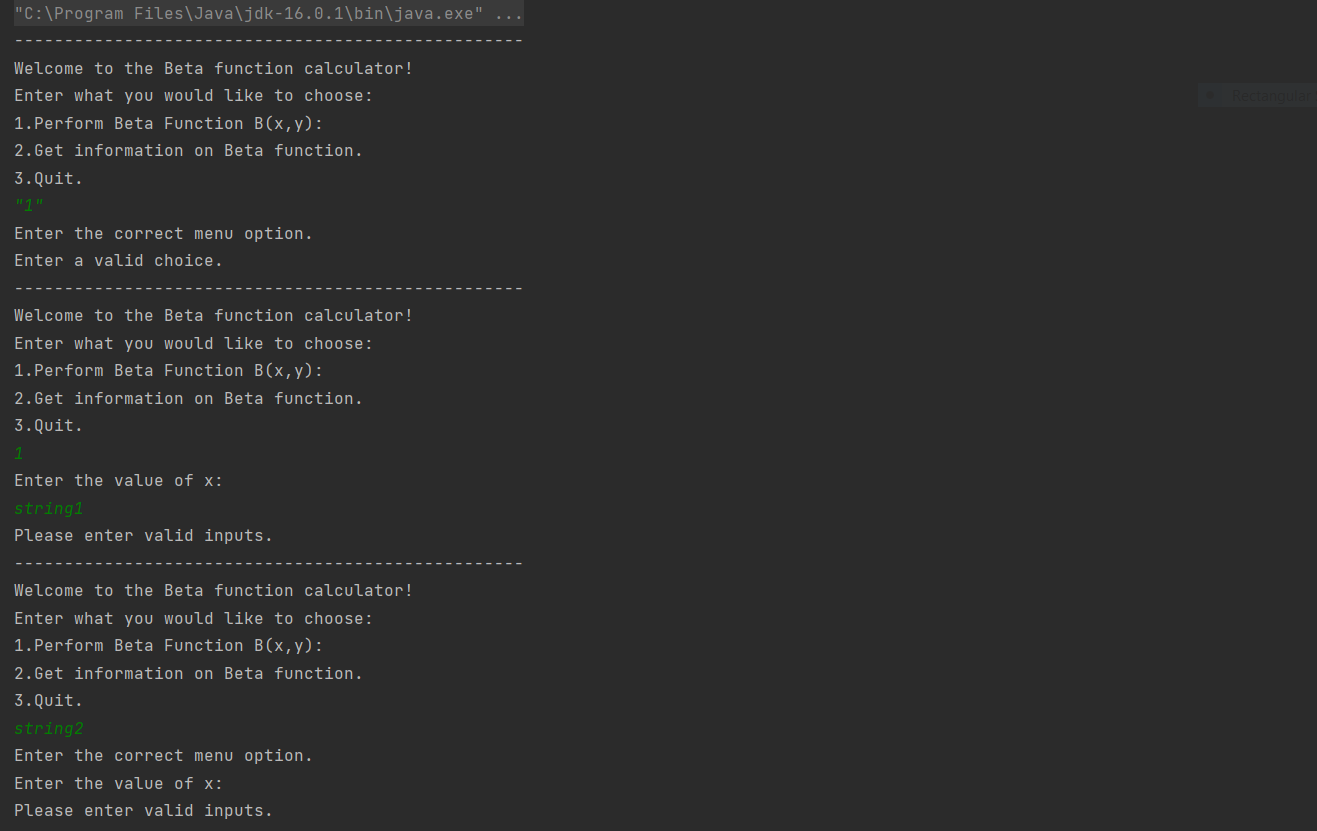
\includegraphics[width=18cm]{images/error1.PNG}
        \end{center}
        \caption{Error Handling for wrong menu option}
        \label{fig:error1}
    \end{figure}
    
    \begin{figure}[htb]
        \begin{center}
            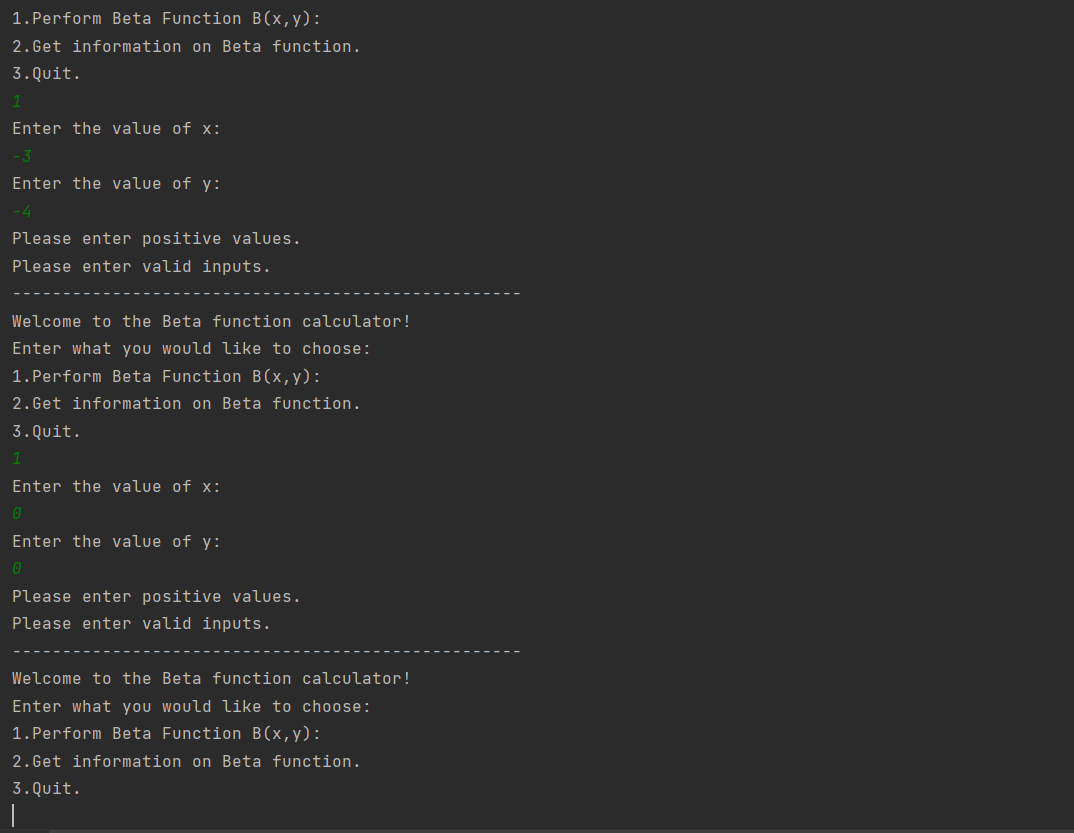
\includegraphics[width=18cm]{images/error2.PNG}
        \end{center}
        \caption{Error Handling for wrong inputs}
        \label{fig:error2}
    \end{figure}

\subsection{Debugger}
   \subsubsection{Description:}
    In this project, the debugger used is a built in IntelliJ debugger. A debugger is a tool for finding all the  bugs and trying to identify what's happening  in the underlying parts of the code. To debug, set breakpoints in the code  where you want to pause the program’s execution and examine the program’s state and behavior. On setting the breakpoints, you are all set to debug. You’ll find the results in the Debug tool window in figure \ref{fig:debug1}. \cite{Debugger1}

    \subsubsection{\textbf{Advantages}}
    \begin{itemize}
        \item In IntelliJ debugging mode, function's variable can be changed.
        \item It provides Breakpoints which cane be added easily by pressing on the left side of the code which also increase the efficiency of debugging.  
        \item By using IntelliJ debugger, one can debug not only in java but also in many other languages.
        \item When you debug your code, the IDE shows you variable values in the source code next to their usages and lets you change the values. You dont need to refer to only to the debug window for doing the same.
        \item You can also use the Smart Step-Into action features to debug  the specific method call you want.
        \item The IntelliJ has good debugging support.
        \item Easy to evaluate indiviual terms of series and check for accuracy and see whats going wrong, and where the approximations are slowly causing the result to become inaccurate.
        \item Evaluation of mathematical expressions are easier.
        \item Extremely customized break point features\cite{Debugger2}.
     \end{itemize}

    \subsubsection{\textbf{Disadvantages}}
    \begin{itemize}
        \item Some programs have multi-threading, which makes it more complicated to control the program.
        \item The debugger can be slow and can take time to step into functions and jump as compared to other IDE's.
        \item Makes the debugging of function which have recursion very hard to keep track.
        \item On using manual suspension instead of breakpoints, the debugger can get frozen and not work as required.
        \item Steep learning curve for some users
        \item Debugger window tool can get a bit overwhelming and and inefficient to use with too many options in User interface.
    \end{itemize}
    
    \begin{figure}[htb]
        \begin{center}
            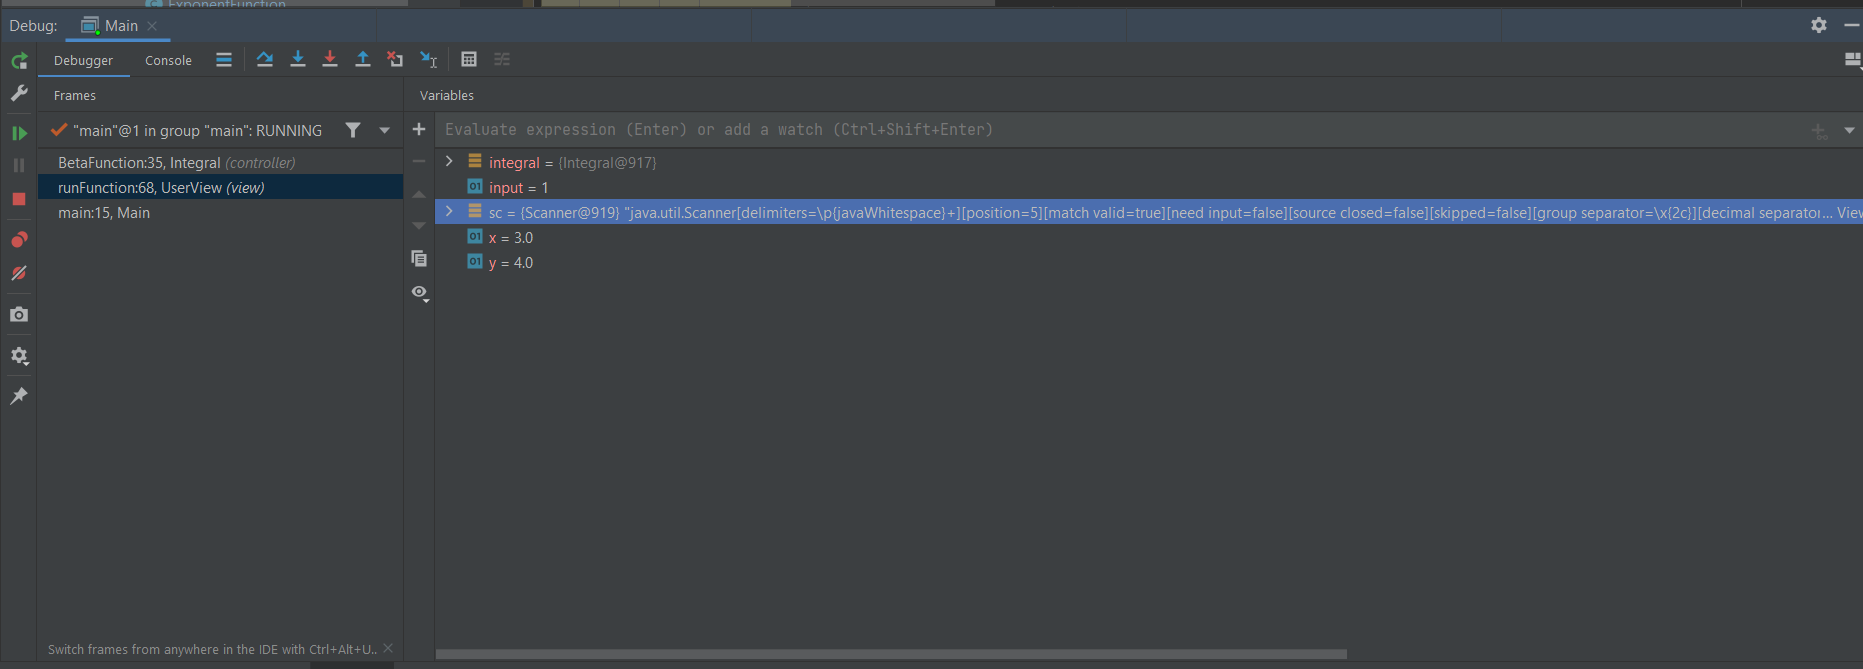
\includegraphics[width=18cm]{images/debugg1.PNG}
        \end{center}
        \caption{Debugging using IntelliJ debugger}
        \label{fig:debug1}
    \end{figure}

    \subsection {Programming style}
    \begin{figure}[htb]
        \begin{center}
            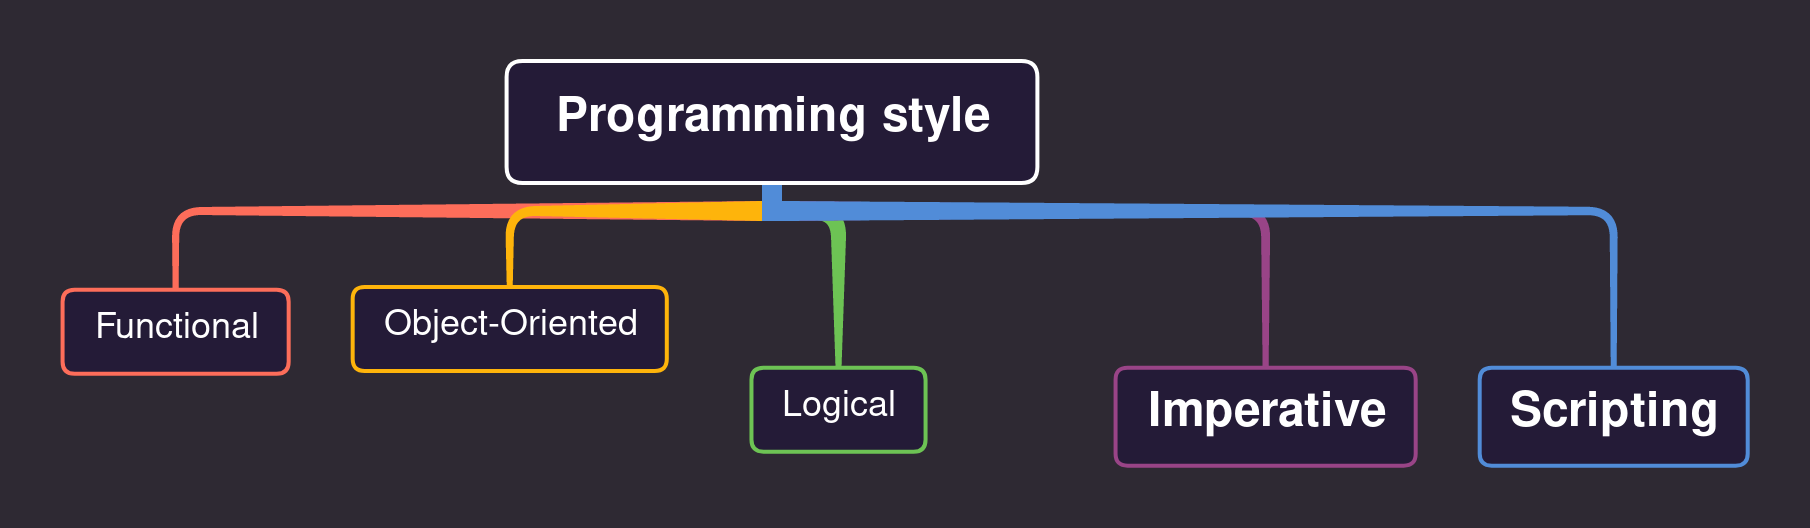
\includegraphics[width=18cm]{images/mindmap_program.png}
        \end{center}
        \caption{Mind map for Programming style decision}
        \label{fig:mindmap}
    \end{figure}
    
    The different programming styles are shown in the mind map above in figure \ref{fig:mindmap}. The Eternity project uses the Object-oriented paradigm using its key features like Data abstraction, Encapsulation and modularization. 
    Other good coding practises have been followed throughtout the project

    
    \subsection{Quality Attributes}
        \begin{itemize}
          \item \textbf{Correctness:} Ensuring to use the correct Exponent function to ensure to get the accurate answers in the definite integral.
          The taylor series for approximating the power function , has a test with different number of iterations ranging from 10 to 100. Based on the tests conducted, the  conclusion is  that to have minimum difference between expected output and actual output , the number of iterations needed is 13.
          \item \textbf{Efficiency:} As the project eternity, the beta calculator in general, uses  many repetitions of mathematical equations which increases the program execution time. As the algorithm mentioned in this paper does not use any complex function structure, it does not show any complexity and can compile quickly.
          \item \textbf{Maintainability:} Usage of javadoc, which provides both readability and maintainability,  and can be used for future references. The project keeps in mind the separation of concerns and has kept all the functionalities as modular as possible which helps to be reused or refactored without breaking any code. Unit test cases are also provided to keep existing functions as before.
          \item \textbf{Robustness:} Error handling, which shows appropriate messages on entering wrong inputs, keeps the project from crashing and can ensure smooth experience for user without any interruption.
          \item \textbf{Usability:} The project is in an executable jar file so that other users can use my file without any difficulties. The user need not worry about the implementation details. The Command line interface also provides step by step instructions on performing the Beta calculations.
        \end{itemize}
  
    \subsection{Checkstyle} 
    Checkstyle - plug-in for IDE's is used to check the quality of any source code. Checkstyle is mainly used to improve the formation of the code and ensure the code follows good programming practices. It has Sun and Google-style support, and I choose the Google-style support. It can automatically generate the issues of the code. Most parameters and constants were subsequently changed to be final since they are not modified in the function body, lines were split to not exceed too many characters, and an else statement was moved to the same line as the preceding bracket. The class was also given an empty private constructor to ensure it could never be instantiated due to it being a static utility/library class.\cite{Checkstyle}
    \subsubsection{\textbf{Advantage:} }
    \begin{itemize}
        \item Checkstyle is mainly used to improve the formation of the code. It has a simple installation process. It can automatically generate the issues of the code. It helps the programmer adhere to good programming and coding practises.
        \item The Checkstyle has good support in case of any errors during installation. 
        \item It automates the process of checking Java code to spare humans of this boring (but important) task.
        \item This makes it ideal for projects that want to enforce a coding standard.
        \item Checkstyle is highly configurable and can be made to support almost any coding standard.
        \item Checkstyle is portable across different IDE's like Eclipse and IntelliJ.
    \end{itemize}
    \subsubsection{\textbf{Disadvantage:}}
        \begin{itemize}
            \item There is less space between the 'error,' 'warnings'  and 'description,' 'resource' and 'path,' less space, making it challenging to understand the problem correctly. Can be ambiguous in some situations.
            \item The only two noticeable annoyances were the inconsistencies in style being labelled as \textit{errors} instead of \textit{warnings}, and that the way the lines with these \textit{errors} were highlighted by Eclipse and/or Checkstyle made it difficult to find issues like an extra space.
            \item Checkstyle can be very efficient but in the mean time can also suggest code changes which are not of high priority. And hence can be a waste of time reorganising code.
        \end{itemize}
    \pagebreak

\section{Annexure:}
    \begin{itemize}
      \item \textbf{Trello Board :} \textit{https://trello.com/eternity119}
      \item \textbf{Code Version Control :} \textit{https://github.com/neonapinto/Scientific\_calculator}
      \item \textbf{Overleaf :} \textit{https://www.overleaf.com/project/62ec550934d66385ad8d07ee}
    \end{itemize}
    
\pagebreak

\begin{thebibliography}{}      
\bibitem{UniversityLogo} 
Concordia Logo : The logo of Concordia University with transparent background
\\\texttt{https://www.pngwing.com/en/free-png-djpzn}

\bibitem{Debugger1}
IntelliJ Features
\\\texttt{https://www.trustradius.com/products/intellij-idea/reviews}

\bibitem{Debugger2} 
JetBeans Features
\\\texttt{https://www.jetbrains.com/idea/features/}

\bibitem{Checkstyle} 
Checkstyle Features
\\\texttt{https://stackoverflow.com/questions/26955766/intellij-idea-checkstyle}



\end{thebibliography}  
\end{document}